\chapter{Implementation}

%Explain what you did to implement your solution, problems that occurred and how you fixed them. 
%If they are interesting, include some relevant parts of the implementation (most relevant pieces of code and so on). 

\section{Communication Protocols}


Centralized pool, robots, charging stations and sensors need to share information with each other.
To improve the communication efficiency, communication protocols are designed. 

\subsection{Message about Measurement}
\label{sec:measurement_message}
When a robot passes by a door, it should receive messages from a sensor. In this project, we use a ROS node "sensor simulator" to simulate door sensors (Section \ref{sec:sensor_simulatior}) to publish instant measurement result (Table \ref{tab:sensor_message}).

\begin{table}[htb]
\centering
\begin{tabular}{|c|c|c|c|c|} 
\hline
Door ID  & Position& Timestamp & Measurement Result \\
\hline\hline
1&(-18.5,5.2) & 2020-06-01 9:00:02 & Door opened \\ [1ex] 
\hline
\end{tabular}
\caption{Measurement Message Format and Example}
\label{tab:sensor_message}
\end{table}
	

\subsection{Message about Task}
\label{sec:task_message}
There are some basic requirements for communication between robot and centralized pool: firstly,
robot should initiate the communication once it has finished all task in task queue and get free. 
Secondly, robot should forward sensor data to centralized pool while processing a task. 
These Communication protocols save unnecessary communication cost by avoiding keep tracking the current position, availability and states of all robots (Figure \ref{fig:comminication}).
Four types of message are defined: 
(1)Task request message(Table\ref{tab:request_message}); (2) Task goal messages(Table \ref{tab:goal_message}); (3) Task feedback message (Table \ref{tab:feedback_message}); (4) Task result message (Table \ref{tab:result_message}). 

\begin{figure}[htbp]
    \centering
    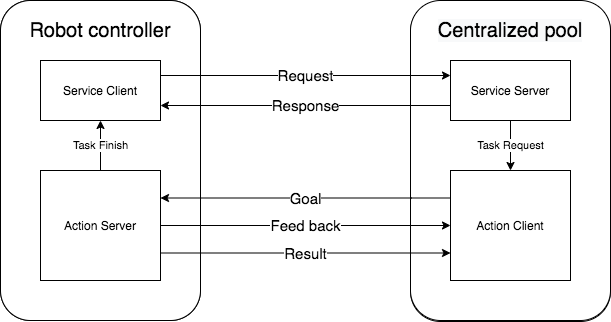
\includegraphics[width = 0.7\textwidth]{content/images/ch4/robot_pool_comminication.drawio.png}
    \caption{Communication between Robot and Centralized Pool}
    \label{fig:comminication}
\end{figure}

\begin{table}[htb]
\centering
\begin{tabular}{|c|c|c|} 
\hline
Battery Level & Position & Robot ID\\
\hline\hline
93	&(2,4)	&1 \\ [1ex] 
\hline
\end{tabular}
\caption{Request Message Format and Example}
\label{tab:request_message}
\end{table}

\begin{table}[htb]
\centering
\resizebox{\textwidth}{!}{
\begin{tabular}{|c|c|c|c|} 
\hline
Task ID-[] &Task type & Target ID & Goal[] \\
\hline\hline
1& Gather Environment Info & 9	& (-1.5,5.2) 2020-06-01 9:00:00 \\
\hline
[3,4]	& Execute task & 21, 22	& (-24.0,12.0), 2020-06-01 9:02:00 (-21.0,12.0) 2020-06-01 9:02:00 \\
\hline
5	& Charging	& 17	&(0.0,5.0), 2020-06-01 9:04:00 \\ [1ex] 
\hline
\end{tabular}}
\caption{Action Goal Message Format and Example}
\label{tab:goal_message}
\end{table}

\begin{table}[htb]
\centering
\begin{tabular}{|c|c|c|c|} 
\hline
Robot ID & Door ID & Measurement time & Measurement result \\
\hline\hline
1	& 3	& 2020-06-01 9:00:03 & Door open \\ [1ex] 
\hline
\end{tabular}
\caption{Action Feedback Message Format and Example}
\label{tab:feedback_message}
\end{table}

\begin{table}[htb]
\centering
\begin{tabular}{|c|c|c|} 
\hline
Task ID 	& Task type	& Result\\
\hline\hline
1 & Gather Environment Info & Success \\ [1ex] 
\hline
\end{tabular}
\caption{Action Result Message Format and Example}
\label{tab:result_message}
\end{table}


\begin{table}[htb]
\centering
\begin{tabular}{|c|c|c|} 
\hline
Robot ID & Battery Level \\
\hline\hline
1 & 93 \\ [1ex] 
\hline
\end{tabular}
\caption{Message to Charging Station}
\label{tab:message_to_charging_staion}
\end{table}

\subsection{Message about Charging}
  
When a robot arrives charging station's position, it sends a message to Charging station(Figure \ref{tab:message_to_charging_staion}). The details of charging station is discussed in Section \ref{sec:charging_station}. 

\section{Database}
The centralized pool keep environment information in database to make decisions. The structure of database is shown in Figure \ref{fig:database_er}.

\begin{figure}[htbp]
\centering
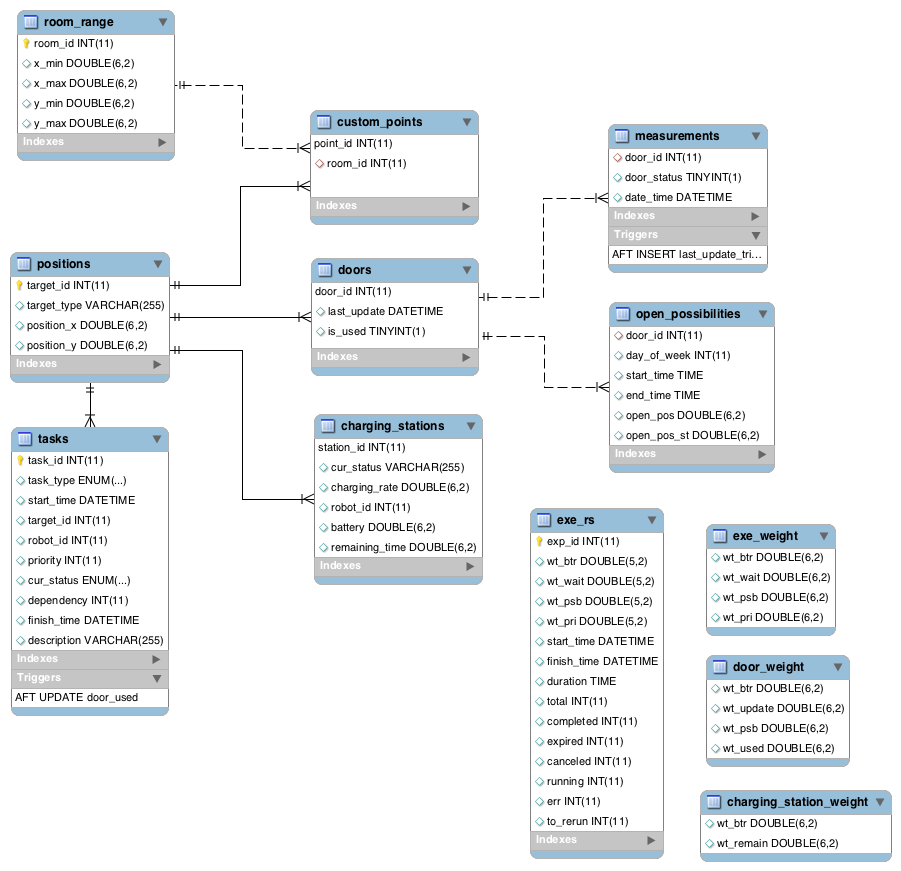
\includegraphics[width = 0.8\textwidth]{content/images/ch4/database_er.png}
\caption{Database Entity Relationship Diagram}
\label{fig:database_er}
\end{figure}

\begin{table}[htb]
\centering
\begin{tabular}{|c|c|c|} 
\hline
Table Name & Example & Explaination \\ \hline
measurements & Table \ref{tab:db_measurement_result}  & measurement result with timestamp \\ \hline
doors   & Table \ref{tab:db_doors} & door information \\ \hline
tasks & Table \ref{tab:db_task_table} & task specifications  \\ \hline 
exe\_rs  & Table \ref{tab:exp_decision_variables} & ``execute task'' experiment result \\ \hline
env\_rs & Table \ref{tab:enviroment_experiment_result} & ``gather enviroment information task'' experiment result \\ \hline
open\_possibilities & Table \ref{tab:db_open_possibilities} & open possibilities table for different time slots and weekdays \\ \hline
... & ... & ... \\ \hline
\end{tabular}
\caption{Tables in Database}
\label{tab:tables_in_database}
\end{table}



\section{Procedure}
\label{sec:task_allocation_procedure}
As stated in the Chapter 3, the goal of task scheduling is finishing all tasks as soon as possible while keep the cost as low as possible. 
The task assignment and execution has at two level. \cite{Ivan2017} the task and the path planner solves a planning problem. It takes and occupancy grid, a specific robot and a set of task specifications, and generates trajectories for each task under the assumption that there are no dynamic obstacles (include other robots). According to those trajectories and task specifications, the task with the lowest cost will be assigned to robot.
At the dynamic level, after each robot receive a task, it runs a navigation stack to execute this task stepwise. Each robot computes a local trajectory but takes into account dynamic obstacles.
The process of the robot task allocation system is as follows.

\begin{figure}[htbp]
    \centering
    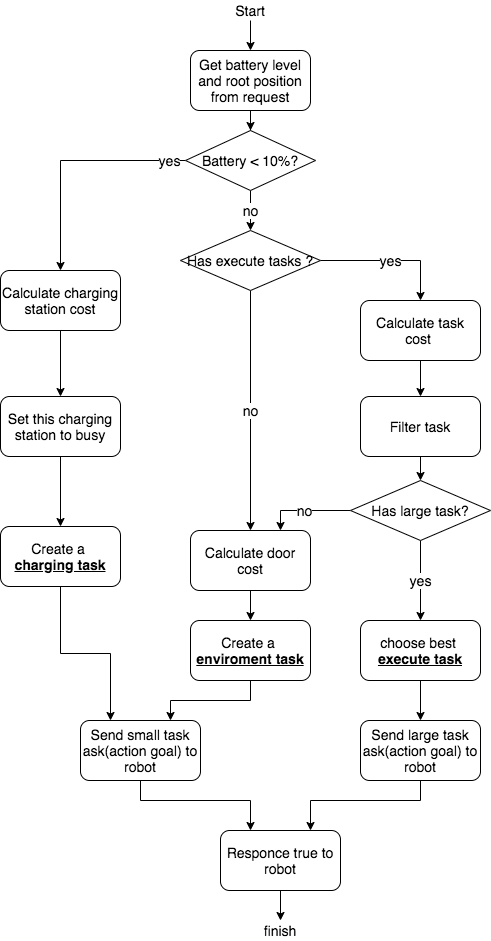
\includegraphics[width = 0.7\textwidth]{content/images/ch4/centralized_task_select.drawio.png}
    \caption{Centralized Pool Task Allocation}
    \label{fig:centralized_task_allocation}
\end{figure}

\subsection{Centralized Pool}
With robot status such as positions and available battery provided by robot, the multi-robot task allocation module in the architecture should perform multi-robot task allocation. 
When the centralized pool receives a task request (Table \ref{tab:request_message}) from robot,  the multi-robot task allocation module in the architecture. The implementation of task allocation is shown in Figure \ref{fig:centralized_task_allocation}. 

The process of task allocation is shown in Figure \ref{fig:centralized_task_allocation}. 

\paragraph{Handle Task Feedback.}
When the centralized pool receives a task feedback (Table \ref{tab:feedback_message}) that contains a new measurement result from robot, it will add a record in ``measurement table'' and update ``open possibilities table'' in database (Table \ref{tab:db_open_possibilities}).

\begin{table}[htb]
\centering
\begin{tabular}{|c| c| c|} 
\hline
Door ID & Door Status & Date Time \\
\hline
9 & 1 & 2020-06-01 09:05:39 \\ \hline
1 & 0 & 2020-06-01 09:05:49 \\ \hline
7 & 1 & 2020-06-01 09:05:49 \\ \hline
9 & 1 & 2020-06-01 09:05:49 \\ \hline
1 & 1 & 2020-06-01 09:05:59 \\ \hline
7 & 1 & 2020-06-01 09:05:59 \\ \hline
9 & 1 & 2020-06-01 09:05:59 \\ \hline
7 & 1 & 2020-06-01 09:06:09 \\ \hline
16 & 0 & 2020-06-01 09:06:29 \\ \hline
7 & 1 & 2020-06-01 09:06:39 \\ \hline
16 & 1 & 2020-06-01 09:06:39 \\ \hline
9 & 1 & 2020-06-01 09:06:49 \\ \hline
8 & 0 & 2020-06-01 09:06:59 \\ \hline
... & ...& ... \\ \hline
\end{tabular}
\caption{Measurement Result Table}
\label{tab:db_measurement_result}
\begin{itemize}
    \item \textsl{Column Door ID.} Unique identification of the door.
    \item \textsl{Column Door Status.} Value 0 represent door closed. Value 1 represent door opened.
    \item \textsl{Column Date Time.} Measuring time.
\end{itemize}

\end{table}

\begin{table}[htb]
\centering
\resizebox{\textwidth}{!}{
\begin{tabular}{|c|c| c| c| c| c|} 
\hline
Door ID & Day Of Week & Start Time & End Time & Initialized Open Possibility &  Open Possibility Statistic \\ \hline
1 & 2 & 9:00:00 & 9:59:59 & 0.90 & 0.85 \\ \hline
1 & 2 & 10:00:00 & 10:59:59 & 0.90 & 0.92 \\ \hline
1 & 2 & 11:00:00 & 11:59:59 & 0.10 & 0.05 \\ \hline
...&...& ...&...&...&...\\ \hline
\end{tabular}}
\caption{Door Open Possibility}
\label{tab:db_open_possibilities}
\begin{itemize}
    \item \textsl{Column Door ID.} Unique identification of the door. 
    \item \textsl{Column Day of Week} a weekday.
    \item \textsl{Column Start Time and End Time} a time slot between start time and end time.
    \item \textsl{Column Initialized Open Possibility} Predefined value to used to simulate door sensors (Section \ref{sec:sensor_simulatior}).
    \item \textsl{Column Open Possibility Statistic} Statistics of measurement result in the weekday and time slot.
\end{itemize}
\end{table}


\paragraph{Handle Task Result.}
When the centralized pool receives a task result (Table \ref{tab:result_message}), it updates status column in ``tasks'' table in database. Figure explaination of task status:

\begin{itemize}
    \item \textsl{Succedded.} Robot successfully moved to the goal position and complted the task.
    \item \textsl{Error.} An error that cannot be corrected by itself occurred and the system requires manual restart. For example, a robot failed charging.
    \item \textsl{Failed.} A Task failed. Reasons of task failure includes: The robot was not able to move to goal positions or process robot action(\ref{fig:system_architecture}). 
    \item \textsl{To rerun.} If an ``execute task'' failed, its priority was increased. The task is marked as ``to rerun task''  for a future allocation by task allocation module.
\end{itemize}


The failed ``execute tasks'' will be reused while others will be marked as ``Cancel'' or ``Error''(Figure \ref{fig:centralized_task_handle}).



\begin{figure}[htbp]
    \centering
    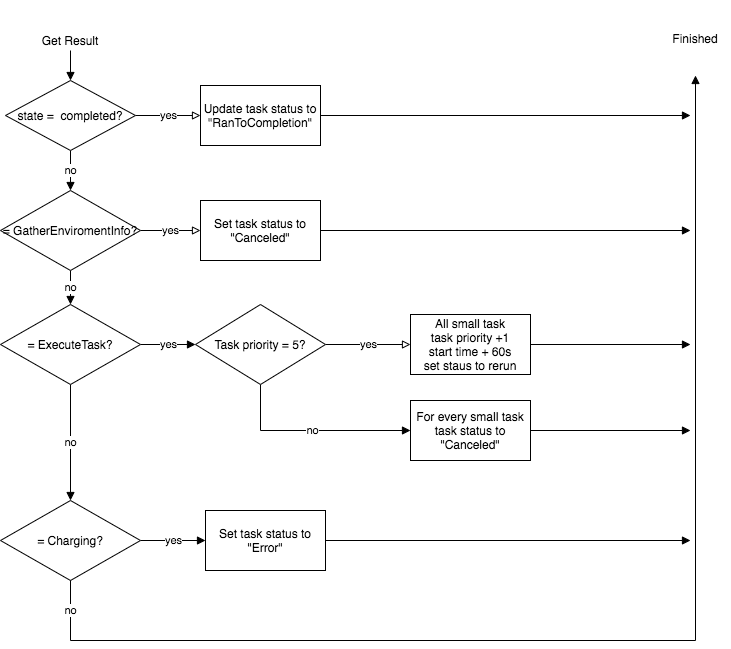
\includegraphics[width = 0.7\textwidth]{content/images/ch4/centralized_task_result.drawio.png}
    \caption{Centralized Pool Handle Task Result}
    \label{fig:centralized_task_handle}
\end{figure}


\subsection{Robot}

\begin{figure}[htbp]
    \centering
    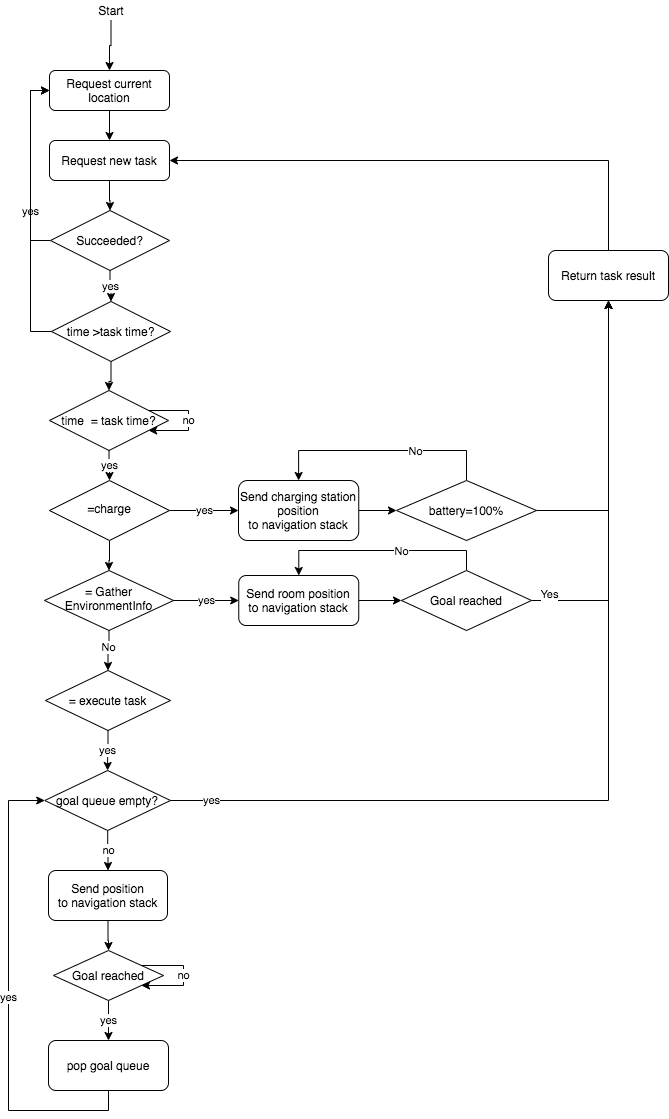
\includegraphics[width = 0.7\textwidth]{content/images/ch4/robot_process_task.drawio.png}
    \caption{Robot Process Task }
    \label{fig:task_process_robot}
\end{figure}

\paragraph{Robot Process Tasks}
When the task queue(Figure \ref{fig:system_architecture}) in a robot is empty, the robot requests a new task. If the robot gets a ``charging task'', it will move to the position of charging staion(Figure \ref{fig:positions_door_station}) and interact with charging station node (Section \ref{sec:charging_station}).
When a robot gets an ``execute task'' which is a complex task, it will move to all goals in order.
When a robot gets a ``gather environment information'' task, it will move to the door's position.
During task processing, the timer checks periodically the status of navigation stack. If any errors occurs, the robot send a ``failed'' result with description to the centralized pool.  
When all tasks are complted without error, the robot will send ``Succedded'' result to the centralized pool.


\begin{figure}[htbp]
    \centering
    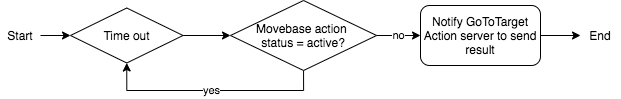
\includegraphics[width = 0.7\textwidth]{content/images/ch4/robot_timer.drawio.png}
    \caption{Robot Timer}
    \label{fig:robot_timer}
\end{figure}

\begin{figure}[htbp]
    \centering
    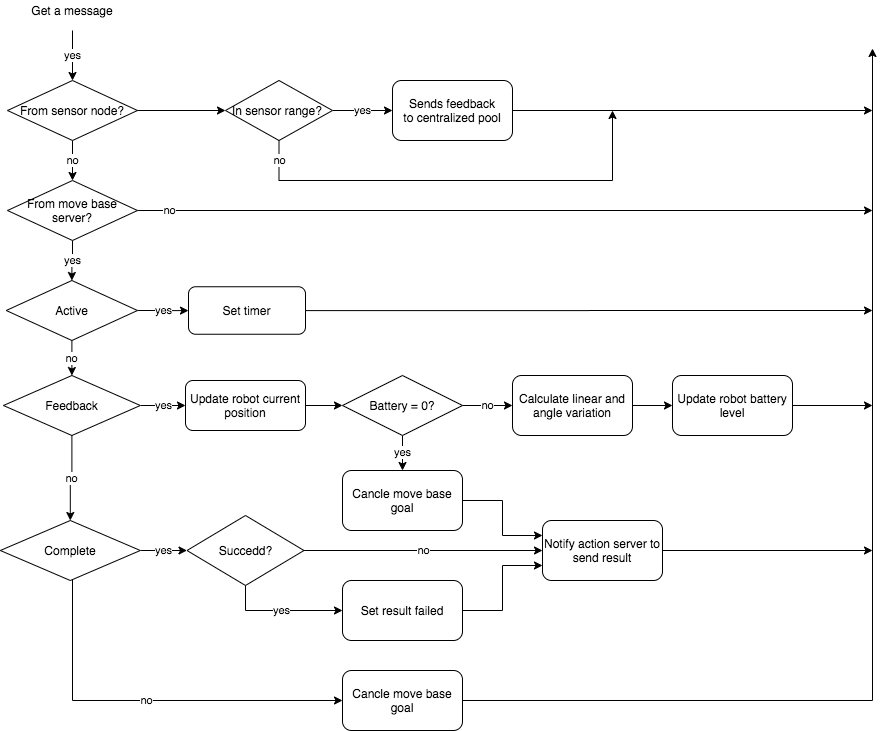
\includegraphics[width = 0.7\textwidth]{content/images/ch4/robot_message.drawio.png}
    \caption{Robot Handle Message}
    \label{fig:robot_handle_message}
\end{figure}

\paragraph{Robot Handle Messages}
While a robot is processing a task, it listens to door sensors and forwards measurement result to the centralized pool. 
Besides messages from sensor, it also receives messages from ``move\_base'' node. The details of robot message handling is shown in Figure \ref{fig:robot_handle_message}.

\subsection{Charging Station}
\label{sec:charging_station}
The charging station consists of a charging station node and ``charging station'' table in database (Table \ref{fig:database_er}). 

A charging station has four states : ``Fre'', ``Charging'' and ``Charging finishe''. Its initial state is "Free". When a robot arrives the position of charging station, it will start interacting with charging station node (Figure \ref{fig:charging_station_message}). 
Once the charging station receives robot information, its state will be changed to ``Charging'' and its ``battery level'' will be increased and its ``remaining time'' will be decreased(Figure \ref{fig:charging_station_event}).  
Once finishing charging, its status will be set to ``Charging finished''. When robot leaves charging station, its status will be set to ``Free''. 

\begin{figure}[htbp]
    \centering
    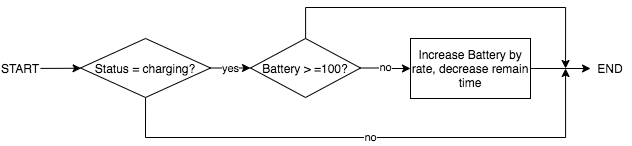
\includegraphics[width = 0.7\textwidth]{content/images/ch4/charging_station_charging_event.drawio.png}
    \caption{Charging Station Scheduled Charging Event in Database}
    \label{fig:charging_station_event}
\end{figure}

\begin{figure}[htbp]
    \centering
    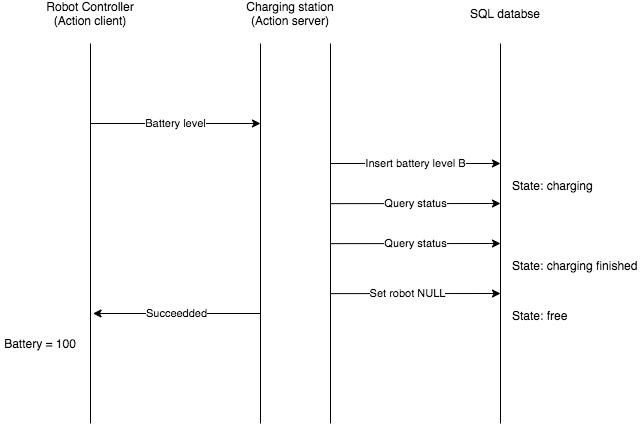
\includegraphics[width = 0.9\textwidth]{content/images/ch4/charging_station_message.drawio.png}
    \caption{Charging Station Message}
    \label{fig:charging_station_message}
\end{figure}
